\section{Data}
\labsec{data}

The Genotype-Tissue Expression (GTEx) project \sidecite{Lonsdale2013a} 
aims to characterise gene expression and regulation for 54 human healthy 
tissues across nearly 1000 people. While the results of the analyses are 
open-access, in order to gain access to the raw data about the DNA and 
the gene expression of the individuals, it is necessary to go through a 
long bureaucratic procedure.

Another source of data was the Ensembl project (release 75), 
\sidecite[-1.55cm]{Zerbino2018} which was used to obtain the coordinates 
of the regulatory regions for each gene. Regulatory regions are 
particular positions around a gene where transcription factors can bind; 
from there, these transcription factors exert a control on gene 
expression.\sidenote{In this project, I considered 141 genes of a 
particular type of blood cells, for 95 individuals. Each gene is 
associated to about 10 regulatory regions on average.} Each 
transcription factor recognises a specific sequence of DNA, therefore it 
is possible to compute the affinity of a factor for a given region. The 
total binding affinity (TBA) \sidecite[-3.85cm]{Molineris2011a} is one 
of the possible affinity measures.\sidenote[][]{The TBA is also 
related to the name of this project, T-REx: indeed, the goal is to 
estimate the TBA-Regulated Expression.}

Gene expression in GTEx was measured with a technique called 
RNA-sequencing, which returns, for each gene and each individual, the 
RPKM, \sidecite[-4.6cm]{Mortazavi2008} which is the number of sequencing 
reads normalised by the length of the gene and by the total number of 
reads.

%\begin{figure}[H]
\begin{figure}[H]
  \begin{subfigure}{\textwidth}
	\centering
	\caption{}
%	\caption{Histogram and normal Q\babelhyphen{nobreak}Q plot of the 
%expression of a randomly selected gene called BID. In the histogram, the 
%brown dashed line indicates the mean, while the dotted lines indicate 
%plus and minus one standard deviation. In the Q\babelhyphen{nobreak}Q 
%plot, each point represents an individual.}
	\labfig{distrexpr}
	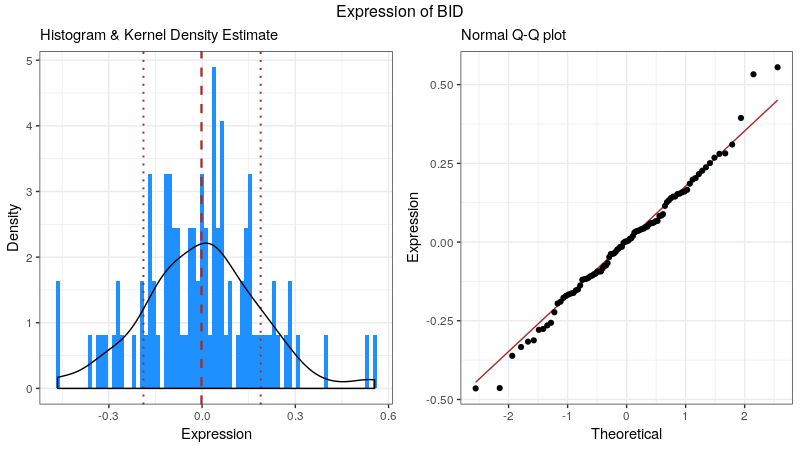
\includegraphics[height=4.8cm,width=.8\textwidth,keepaspectratio=false]{bid_expr}
  \end{subfigure}
%\end{figure}

  \begin{subfigure}{\textwidth}
%\begin{figure}[t]
    \centering
    \caption{}
% 	\caption{Scree plot and biplot of 
% the \textasciitilde800 affinities for the gene BID. In the biplot, each 
% label corresponds to an individual.}
    \labfig{pcatba}
    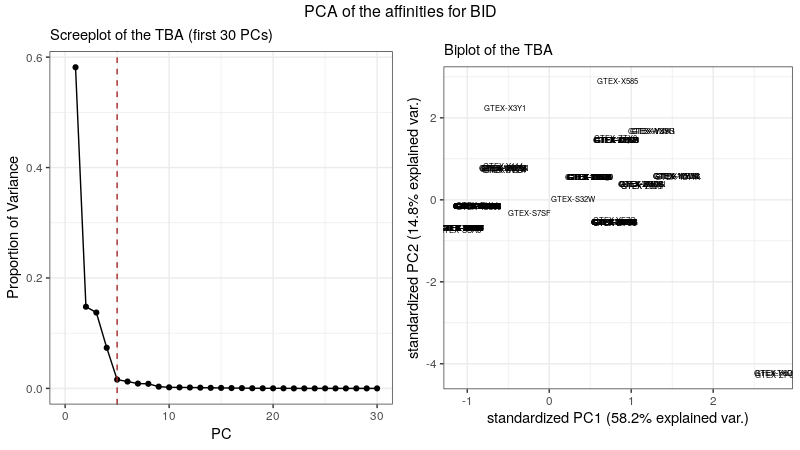
\includegraphics[height=4.8cm,width=.8\textwidth,keepaspectratio=false]{bid_tba}
  \end{subfigure}
% \end{figure}
  \caption{(a): Histogram and normal Q\babelhyphen{nobreak}Q plot of the 
expression of a randomly selected gene called BID. In the histogram, the 
brown dashed line indicates the mean, while the dotted lines indicate 
plus and minus one standard deviation. In the Q\babelhyphen{nobreak}Q 
plot, each point represents an individual. (b): Scree plot and biplot of 
the \textasciitilde800 affinities for the gene BID. In the biplot, each 
label corresponds to an individual.}
  \labfig{expl}
\end{figure}

The expression was preprocessed as recommended by the Stephen's 
Lab.\sidenote[][*7]{\url{http://stephenslab.github.io/gtex-eqtls/analysis/20170515\_RNASeq\_Analysis.html}} 
In summary, I applied a quantile normalisation to make sure that the 
distribution of our response variable was normal, and then I obtained 
the residuals of a linear model 
$Y~\sim~SEX+PEER\_FA+POPULATION+PLATFORM$, so as to disregard the 
effects of these covariates on the expression. The final result can be 
seen in \reffig{distrexpr}.

The genotypes were also obtained with a sequencing technique and were 
provided in VCF format. \sidecite[-3.2cm]{Danecek2011} I 
used a software called 
\nohyphens{VCF\textunderscore\nobreak\hspace{0pt}rider}\sidenote[][*3]{\url{https://github.com/vodkatad/vcf\_rider}} 
to compute the total binding affinity of each transcription factor for 
each regulatory region associated to a gene (the total number of 
transcription factors is about 800). \reffig{pcatba} reports the PCA of 
the TBA for the gene BID.
